\chapter{Arhitektura i dizajn sustava}
		
		\textbf{\textit{dio 1. revizije}}\\

		\textit{ Potrebno je opisati stil arhitekture te identificirati: podsustave, preslikavanje na radnu platformu, spremišta podataka, mrežne protokole, globalni upravljački tok i sklopovsko-programske zahtjeve. Po točkama razraditi i popratiti odgovarajućim skicama:}
	\begin{itemize}
		\item 	\textit{izbor arhitekture temeljem principa oblikovanja pokazanih na predavanjima (objasniti zašto ste baš odabrali takvu arhitekturu)}
		\item 	\textit{organizaciju sustava s najviše razine apstrakcije (npr. klijent-poslužitelj, baza podataka, datotečni sustav, grafičko sučelje)}
		\item 	\textit{organizaciju aplikacije (npr. slojevi frontend i backend, MVC arhitektura) }		
	\end{itemize}
		
		\section{Organizacija sustava}
			\subsection{Uvod}
				Arhitekturu sustava čine tri glavna dijela:
				\begin{packed_item}
					\item Baza podataka
					\item Internetski poslužitelj
					\item Aplikacija
				\end{packed_item}
			
				Internetski poslužitelj ključan je dio u uspostavljanju komunikacije između korisnika i aplikacije. Korisnik aplikaciji pristupa pomoću internetskog preglednika na svom računalu, mobitelu ili nekom drugom uređaju. Preglednik komunicira s poslužiteljem preko HTTP protokola slanjem odgovarajućih zahtjeva. Poslužitelj je onaj koji pokreće aplikaciju te joj prosljeđuje korisnikove HTTP zahtjeve.
				\linebreak
				Aplikacija preuzima zahtjev te ga obrađuje sukladno njegovoj vrsti i parametrima. Obrada zahtjeva uključuje i pristupanje bazi podataka kako bi se dohvatili podatci potrebni za rad. Po završetku obrade zahtjeva, aplikacija preko poslužitelja korisniku vraća odgovor.
				\linebreak
				Baza podataka može se nalaziti na istom računalu kao i poslužitelj i aplikacija ili različitom, no komunikacija se uvijeko odvija na isti način, preko preddefiniranih vrata na transportnom sloju i korištenjem odgovarajućeg protokola.
				\begin{figure}[H]
					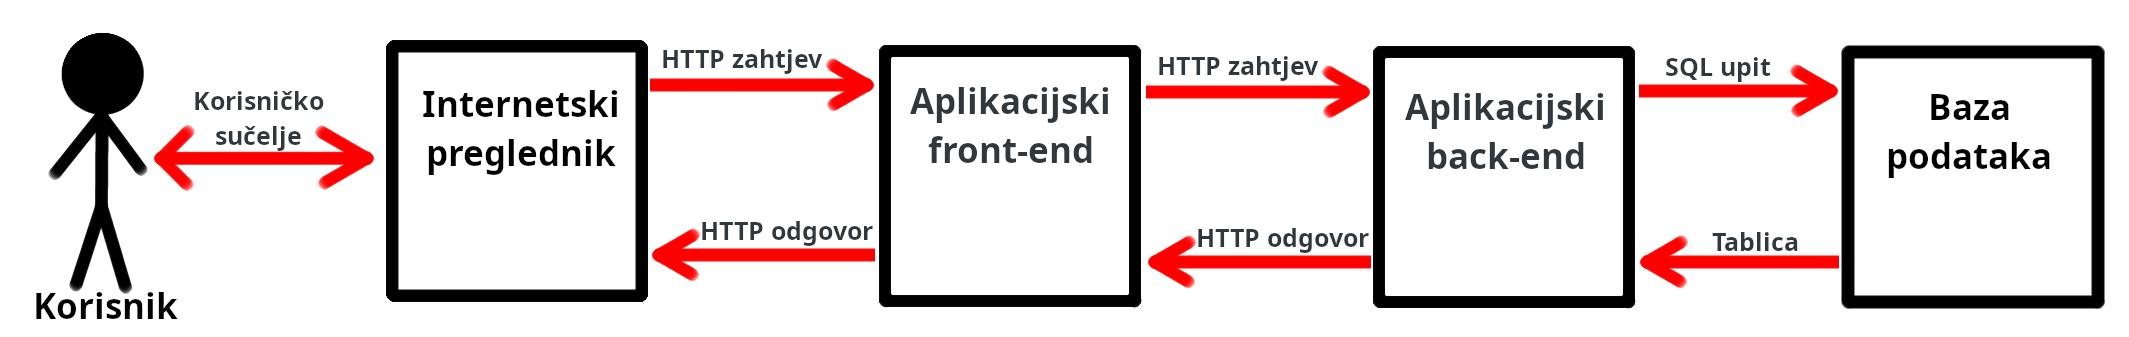
\includegraphics[scale=1]{slike/skica_arhitekture.png}
					\centering
					\caption{Arhitektura sustava}
					\label{fig:arhitektura_sustava}
				\end{figure}
			\subsection{Sklopovski zahtjevi}
				Ukoliko se poslužitelj i baza podataka nalaze na različitim računalima, za optimalan rad ona bi trebala imati odgovarajuće karakteristike. Računalo na kojem će raditi poslužitelj treba imati dovoljnu veliku procesorsku moć kako bi moglo što brže odgovarati na zahtjeve i kako bi više korisnika moglo koristiti aplikaciju bez značajnog usporavanja sustava. Računalo na kojem će se nalaziti baza podataka treba imati dovoljno velike i brze diskove za pohranu podataka, idealno uz neku vrstu zaštite od gubitka podataka u slučaju kvara (na primjer, korištenje RAID sustava ili automatskog redovitog stvaranja sigurnosne kopije). Ako se pak poslužitelj i baza podataka pokreću na istom računalu, ono treba kombinirati prethodno navedene karakteristike.
			\subsection{Organizacija aplikacije}
				Za izradu aplikacije odabrani su programski jezik Java uz razvojni okvir Spring te Javascript i razvojni okvir React. Dva glavna sloja aplikacije su frontend, koji komunicira s korisnikom (Javascript + React) i backend, koji obrađuje HTTP zahtjeve i komunicira s bazom podataka (Java + Spring).
				%U primjeru dokumentacije oni ovdje jos pisu da se arhitektura temelji na MVCu i to dodatno opisuju
				%Ovaj dio bi onda trebali dovrsit kada vidimo sto cemo s time
				
				
		

		\section{Baza podataka}
			
			\textbf{\textit{dio 1. revizije}}\\
			
		\textit{Potrebno je opisati koju vrstu i implementaciju baze podataka ste odabrali, glavne komponente od kojih se sastoji i slično.}
		
			\subsection{Opis tablica}
			

				\textit{Svaku tablicu je potrebno opisati po zadanom predlošku. Lijevo se nalazi točno ime varijable u bazi podataka, u sredini se nalazi tip podataka, a desno se nalazi opis varijable. Svjetlozelenom bojom označite primarni ključ. Svjetlo plavom označite strani ključ}
				
				
				\begin{longtblr}[
					label=none,
					entry=none
					]{
						width = \textwidth,
						colspec={|X[6,l]|X[6, l]|X[20, l]|}, 
						rowhead = 1,
					} %definicija širine tablice, širine stupaca, poravnanje i broja redaka naslova tablice
					\hline \SetCell[c=3]{c}{\textbf{korisnik - ime tablice}}	 \\ \hline[3pt]
					\SetCell{LightGreen}IDKorisnik & INT	&  	Lorem ipsum dolor sit amet, consectetur adipiscing elit, sed do eiusmod  	\\ \hline
					korisnickoIme	& VARCHAR &   	\\ \hline 
					email & VARCHAR &   \\ \hline 
					ime & VARCHAR	&  		\\ \hline 
					\SetCell{LightBlue} primjer	& VARCHAR &   	\\ \hline 
				\end{longtblr}
				
				
			
			\subsection{Dijagram baze podataka}
				\textit{ U ovom potpoglavlju potrebno je umetnuti dijagram baze podataka. Primarni i strani ključevi moraju biti označeni, a tablice povezane. Bazu podataka je potrebno normalizirati. Podsjetite se kolegija "Baze podataka".}
			
			\eject
			
			
		\section{Dijagram razreda}
		
			\textit{Potrebno je priložiti dijagram razreda s pripadajućim opisom. Zbog preglednosti je moguće dijagram razlomiti na više njih, ali moraju biti grupirani prema sličnim razinama apstrakcije i srodnim funkcionalnostima.}\\
			
			\textbf{\textit{dio 1. revizije}}\\
			
			\textit{Prilikom prve predaje projekta, potrebno je priložiti potpuno razrađen dijagram razreda vezan uz \textbf{generičku funkcionalnost} sustava. Ostale funkcionalnosti trebaju biti idejno razrađene u dijagramu sa sljedećim komponentama: nazivi razreda, nazivi metoda i vrste pristupa metodama (npr. javni, zaštićeni), nazivi atributa razreda, veze i odnosi između razreda.}\\
			
			\textbf{\textit{dio 2. revizije}}\\			
			
			\textit{Prilikom druge predaje projekta dijagram razreda i opisi moraju odgovarati stvarnom stanju implementacije}
			
			
			
			\eject
		
		\section{Dijagram stanja}
			
			
			\textbf{\textit{dio 2. revizije}}\\
			
			\textit{Potrebno je priložiti dijagram stanja i opisati ga. Dovoljan je jedan dijagram stanja koji prikazuje \textbf{značajan dio funkcionalnosti} sustava. Na primjer, stanja korisničkog sučelja i tijek korištenja neke ključne funkcionalnosti jesu značajan dio sustava, a registracija i prijava nisu. }
			
			
			\eject 
		
		\section{Dijagram aktivnosti}
			
			\textbf{\textit{dio 2. revizije}}\\
			
			 \textit{Potrebno je priložiti dijagram aktivnosti s pripadajućim opisom. Dijagram aktivnosti treba prikazivati značajan dio sustava.}
			
			\eject
		\section{Dijagram komponenti}
		
			\textbf{\textit{dio 2. revizije}}\\
		
			 \textit{Potrebno je priložiti dijagram komponenti s pripadajućim opisom. Dijagram komponenti treba prikazivati strukturu cijele aplikacije.}